\documentclass[11pt,a4paper]{article}
\usepackage[utf8]{inputenc}
\usepackage[T1]{fontenc}
\usepackage{lmodern}
\usepackage[portuguese]{babel}
\usepackage[a4paper,margin=2.4cm]{geometry}
\usepackage{xcolor}
\usepackage{graphicx}
\usepackage{titlesec}
\usepackage{enumitem}
\usepackage{listings}
\usepackage{tcolorbox}
\usepackage{booktabs}
\usepackage{array}
\usepackage{fancyhdr}
\usepackage{hyperref}
\tcbuselibrary{skins,breakable,listings}

\definecolor{BgCream}{HTML}{FAF8F5}
\definecolor{TextEspresso}{HTML}{4A4238}
\definecolor{NudeTaupe}{HTML}{BFAFA6}
\definecolor{SoftBlush}{HTML}{D9C5B2}
\definecolor{SageMuted}{HTML}{7E8F7C}
\definecolor{ClayWarn}{HTML}{B5795C}
\definecolor{SkyCalm}{HTML}{5E7F9A}

\hypersetup{colorlinks=true, linkcolor=SkyCalm, urlcolor=SkyCalm}

\titleformat{\section}{\color{TextEspresso}\Large\bfseries}{\thesection}{0.6em}{}[{\color{NudeTaupe}\titlerule[0.8pt]}]
\titlespacing*{\section}{0pt}{1.6\baselineskip}{0.9\baselineskip}

\setlength{\parindent}{0pt}
\setlength{\parskip}{0.5cm}
\linespread{1.18}
\setlist[itemize]{itemsep=0.3cm, topsep=0.3cm}
\setlist[enumerate]{itemsep=0.3cm, topsep=0.3cm}

\pagestyle{fancy}
\fancyhf{}
\renewcommand{\headrulewidth}{0pt}
\fancyfoot[C]{\color{NudeTaupe}\small\thepage}

% Terminal: fundo preto, letra branca
\newtcblisting{terminal}{
  listing only, breakable, colback=black, colupper=white, colframe=TextEspresso,
  boxrule=0.8pt, arc=3pt, left=10pt, right=10pt, top=8pt, bottom=8pt,
  before skip=0.45cm, after skip=0.6cm,
  title={\small\bfseries Comando a executar},
  coltitle=white, colbacktitle=TextEspresso, fonttitle=\small\bfseries,
  listing options={basicstyle=\ttfamily\small\color{white}, breaklines=true,
    columns=fullflexible, keepspaces=true, showstringspaces=false}
}

\newtcblisting{saida}{
  listing only, breakable, colback=black, colupper=white, colframe=SageMuted,
  boxrule=0.8pt, arc=3pt, left=10pt, right=10pt, top=8pt, bottom=8pt,
  before skip=0.45cm, after skip=0.6cm,
  title={\small\bfseries Resultado esperado (os valores podem variar)},
  coltitle=white, colbacktitle=SageMuted, fonttitle=\small\bfseries,
  listing options={basicstyle=\ttfamily\footnotesize\color{white}, breaklines=true,
    columns=fullflexible, keepspaces=true, showstringspaces=false}
}

\newtcblisting{ficheiro}[1]{
  listing only, breakable, colback=BgCream, colupper=TextEspresso, colframe=SkyCalm,
  boxrule=0.8pt, arc=3pt, left=10pt, right=10pt, top=8pt, bottom=8pt,
  before skip=0.45cm, after skip=0.6cm,
  title={\small\bfseries Conteúdo do ficheiro \texttt{#1}},
  coltitle=white, colbacktitle=SkyCalm, fonttitle=\small\bfseries,
  listing options={basicstyle=\ttfamily\small\color{TextEspresso}, breaklines=true,
    columns=fullflexible, keepspaces=true, showstringspaces=false}
}

\newtcolorbox{erro}{
  breakable, colback=ClayWarn!9, colframe=ClayWarn, boxrule=0.8pt, arc=3pt,
  left=10pt, right=10pt, top=8pt, bottom=8pt, before skip=0.5cm, after skip=0.6cm,
  title={\small\bfseries Erro possível e resolução},
  coltitle=white, colbacktitle=ClayWarn, fonttitle=\small\bfseries
}

\newtcolorbox{observe}{
  breakable, colback=SoftBlush!30, colframe=NudeTaupe, boxrule=0.8pt, arc=3pt,
  left=10pt, right=10pt, top=8pt, bottom=8pt, before skip=0.5cm, after skip=0.6cm,
  title={\small\bfseries Analisar},
  coltitle=TextEspresso, colbacktitle=SoftBlush, fonttitle=\small\bfseries
}

\newtcolorbox{nota}{
  breakable, colback=SkyCalm!8, colframe=SkyCalm, boxrule=0.8pt, arc=3pt,
  left=10pt, right=10pt, top=8pt, bottom=8pt, before skip=0.5cm, after skip=0.6cm,
  title={\small\bfseries Nota},
  coltitle=white, colbacktitle=SkyCalm, fonttitle=\small\bfseries
}

\newtcolorbox{feito}{
  breakable, colback=SageMuted!10, colframe=SageMuted, boxrule=0.8pt, arc=3pt,
  left=10pt, right=10pt, top=8pt, bottom=8pt, before skip=0.5cm, after skip=0.6cm,
  title={\small\bfseries Verificação antes de avançar},
  coltitle=white, colbacktitle=SageMuted, fonttitle=\small\bfseries
}

\newtcolorbox{leitura}{
  breakable, colback=SkyCalm!6, colframe=SkyCalm, boxrule=0.8pt, arc=3pt,
  left=10pt, right=10pt, top=8pt, bottom=8pt, before skip=0.4cm, after skip=0.6cm,
  title={\small\bfseries Como ler a figura},
  coltitle=white, colbacktitle=SkyCalm, fonttitle=\small\bfseries
}

\newtcolorbox{teoria}{
  breakable, colback=BgCream, colframe=TextEspresso, boxrule=0.8pt, arc=3pt,
  left=12pt, right=12pt, top=10pt, bottom=10pt, before skip=0.5cm, after skip=0.7cm,
  title={\small\bfseries Fundamento teórico},
  coltitle=white, colbacktitle=TextEspresso, fonttitle=\small\bfseries,
  before upper={\setlength{\parskip}{0.35cm}}
}

\newcommand{\passo}[2]{%
  \clearpage
  \begin{tcolorbox}[colback=SageMuted, colframe=SageMuted, coltext=white,
    boxrule=0pt, arc=4pt, left=14pt, right=14pt, top=10pt, bottom=10pt,
    before skip=0pt, after skip=0.6cm]
  {\Large\bfseries Passo #1}\hfill{\large\bfseries #2}
  \end{tcolorbox}
}

\newcommand{\cmd}[1]{\texttt{#1}}

\newcommand{\labtitle}[3]{%
  \thispagestyle{empty}
  \begin{center}
  {\color{NudeTaupe}\rule{\textwidth}{0.5pt}}\\[0.6cm]
  {\LARGE\bfseries\color{TextEspresso} Laboratório #1}\\[0.4cm]
  {\large\color{TextEspresso} #2}\\[0.35cm]
  {\normalsize\color{NudeTaupe} Infraestruturas de Computação na Nuvem \quad|\quad #3}\\[0.5cm]
  {\color{NudeTaupe}\rule{\textwidth}{0.5pt}}
  \end{center}
  \vspace{0.5cm}
}

\begin{document}
\labtitle{07}{Primeiro Contacto com Infrastructure as Code}{Aula 07}

\section*{Objetivo e enquadramento}

A Aula 07 apresenta, no plano teórico, o princípio de Infrastructure as Code, a distinção entre abordagens declarativa e imperativa, a idempotência, a gestão de configuração com o Ansible e o provisionamento com o Terraform. Este laboratório torna esses conceitos observáveis numa máquina virtual construída no computador do próprio aluno, onde o Terraform cria containers, o Ansible os configura e o Ansible Vault protege um segredo.

O trabalho não requer acesso ao servidor da unidade curricular nem a qualquer serviço de nuvem. Destina-se a ser realizado durante a aula, ao ritmo de cada aluno, e \textbf{não constitui trabalho a entregar}. Todo o trabalho decorre numa máquina virtual Ubuntu, criada e apagada com um único comando, de modo que o computador do aluno permanece intacto.

\begin{nota}
O Docker e o Terraform são mais simples de utilizar num núcleo Linux. Por esse motivo o laboratório utiliza uma máquina virtual criada com o \cmd{multipass}, que funciona da mesma forma em Windows, macOS e Linux. Quem utilizar Linux pode executar os passos diretamente no seu sistema, a partir do passo 1.3.
\end{nota}

\section*{Resultados de aprendizagem}

No final deste laboratório, o aluno deve ser capaz de:

\begin{itemize}
  \item Distinguir uma operação imperativa de uma operação declarativa e idempotente.
  \item Escrever e executar um playbook Ansible com tasks, template e handler, e interpretar os resultados \emph{changed} e \emph{ok}.
  \item Observar o \emph{drift} e a sua correção por uma nova execução do playbook.
  \item Usar o Terraform para criar recursos, ler o plano de execução e inspecionar o state file.
  \item Ligar as duas ferramentas, usando um inventory gerado pelo Terraform para configurar com o Ansible os containers criados.
  \item Cifrar um segredo com o Ansible Vault e verificar que não fica legível no repositório.
\end{itemize}

\section*{Requisitos}

\begin{itemize}
  \item Computador com Windows, macOS ou Linux.
  \item Cerca de 4 GB de memória livres para a máquina virtual e 15 GB de espaço em disco.
  \item Ligação à Internet, necessária para obter a imagem, os pacotes e os providers do Terraform.
  \item Permissão para instalar o \cmd{multipass} (Windows e macOS) ou o \cmd{snap} (Linux).
  \item Duração estimada: entre 90 e 120 minutos.
\end{itemize}

\section*{Como utilizar este guião}

Cada passo apresenta, por esta ordem, o objetivo, o enquadramento, o fundamento teórico, os comandos a executar e o resultado esperado. Recomenda-se ler o passo completo antes de executar o primeiro comando. As caixas têm sempre o mesmo significado:

\begin{terminal}
Comando a executar no terminal.
\end{terminal}

\begin{saida}
Resultado que deve ser apresentado.
\end{saida}

\begin{ficheiro}{exemplo.txt}
Conteúdo a gravar num ficheiro, com um editor como o nano.
\end{ficheiro}

\begin{observe}
Momento de pausa para interpretar o resultado obtido, isoladamente ou em discussão com os colegas.
\end{observe}

\begin{erro}
Erro que pode ocorrer e respetiva resolução.
\end{erro}

\begin{nota}
Informação complementar que facilita a execução.
\end{nota}

Os comandos podem ser copiados e colados. Os resultados mostrados são exemplos: identificadores, tempos e números de versão diferem de computador para computador. Os ficheiros são criados em \cmd{\textasciitilde/icn-aula07}, dentro da máquina virtual.

\section*{Percurso}

A figura seguinte resume a sequência do guião. Os passos 4 e 5 constituem a observação central: o Terraform cria os hosts e o Ansible configura-os, ligados por um inventory que o próprio Terraform gera.

\begin{center}
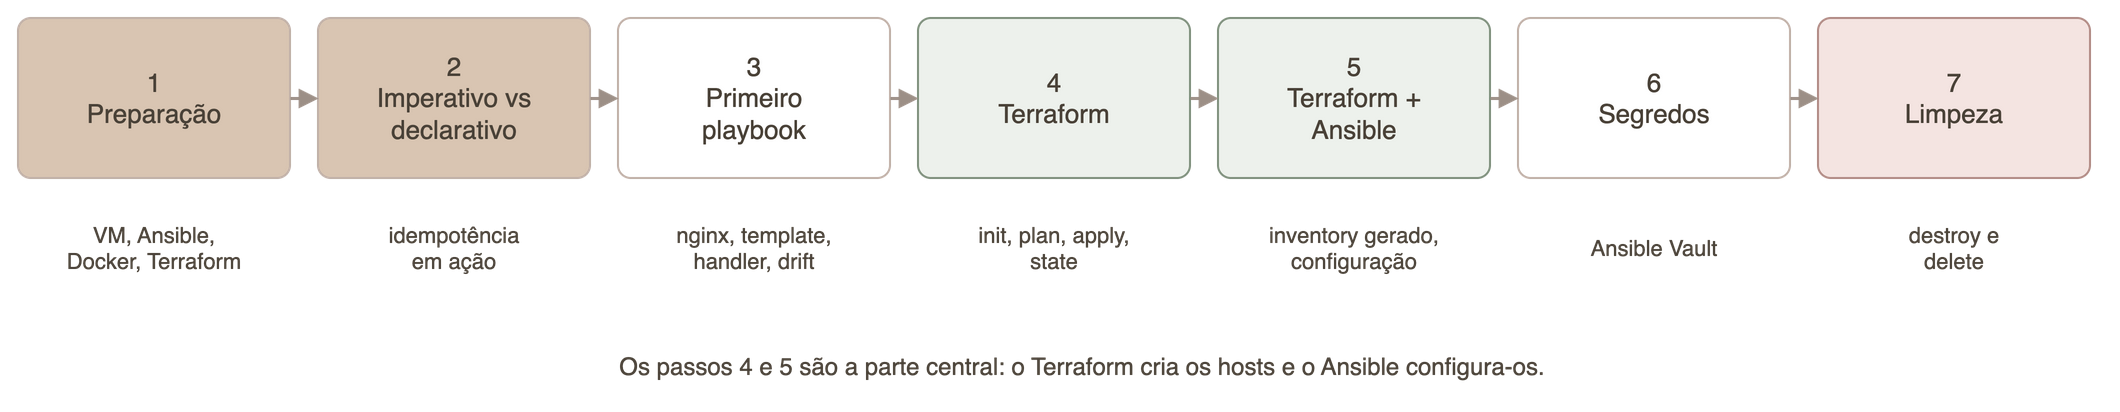
\includegraphics[width=\linewidth]{../Diagramas/g07-percurso.png}
\end{center}

\begin{leitura}
Os sete passos leem-se da esquerda para a direita. Os dois primeiros, a bege, preparam o ambiente e mostram a diferença entre executar passos e declarar um estado. O passo 3, a branco, usa o Ansible sozinho. Os passos 4 e 5, a verde, são a parte central: o Terraform provisiona os containers e o Ansible configura-os. O passo 6, a branco, acrescenta a proteção de um segredo. O passo 7, em tom avermelhado, encerra o trabalho e liberta os recursos. Abaixo de cada caixa, uma legenda resume o que é feito nesse passo.
\end{leitura}

\passo{1}{Preparação do ambiente}

\textbf{Objetivo.} Criar uma máquina virtual Ubuntu e instalar nela o Ansible, o Docker e o Terraform.

\textbf{Enquadramento.} As três ferramentas representam camadas diferentes do que foi estudado na Aula 07. O Terraform provisiona recursos, o Ansible configura o que corre dentro deles e o Docker fornece os recursos que vão ser provisionados, sem exigir um servidor ou uma conta em nenhuma nuvem.

\begin{center}
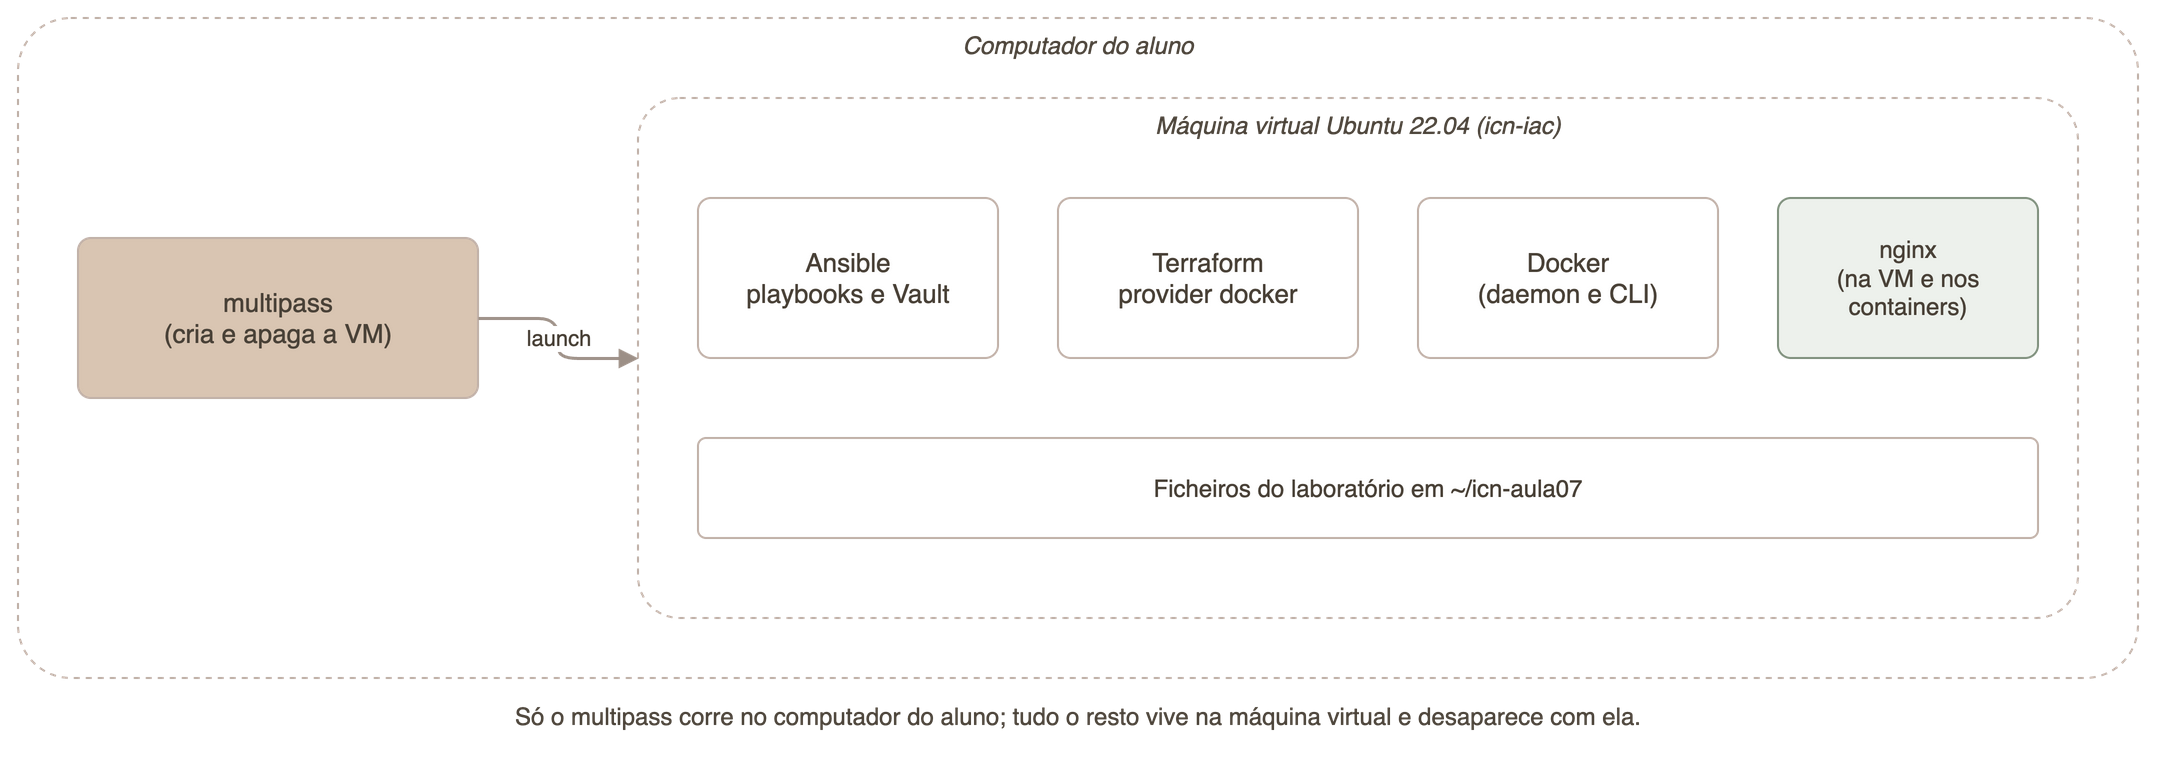
\includegraphics[width=\linewidth]{../Diagramas/g07-ferramentas.png}
\end{center}

\begin{leitura}
A caixa exterior representa o computador do aluno. À esquerda está o \cmd{multipass}, o único programa instalado no computador, cuja função é criar e apagar a máquina virtual. A caixa interior é essa máquina virtual, onde estão as quatro peças do laboratório: o Ansible, o Terraform, o Docker e o nginx, que serve as páginas na máquina virtual e nos containers. Por baixo ficam os ficheiros do laboratório. Tudo o que é instalado fica dentro da máquina virtual e desaparece quando esta é apagada.
\end{leitura}

\begin{teoria}
O Ansible é \emph{agentless}: não exige software residente nos hosts geridos, apenas uma forma de os alcançar. Normalmente essa forma é o SSH. Neste laboratório usam-se também a ligação local, para configurar a própria máquina virtual, e a ligação ao Docker, que executa os módulos dentro de um container com \cmd{docker exec}.

O Terraform, por seu lado, não sabe criar nada sozinho. Delega nos \emph{providers}, plugins que traduzem o código em chamadas à API de cada plataforma. Aqui o provider usado é o do Docker, que fala com o daemon da máquina virtual.

Neste passo, deve analisar-se onde vive cada ferramenta. Apenas o \cmd{multipass} corre no computador do aluno, e tudo o resto corre dentro da máquina virtual.
\end{teoria}

\subsection*{1.1 Instalação do Multipass}

Em macOS, com o Homebrew, executar o primeiro comando. Em Windows, utilizar o instalador disponível em \url{https://multipass.run}. Em Linux, executar o segundo comando.

\begin{terminal}
brew install --cask multipass
\end{terminal}

\begin{terminal}
sudo snap install multipass
\end{terminal}

Confirmar a instalação:

\begin{terminal}
multipass version
\end{terminal}

\begin{saida}
multipass   1.xx.x
\end{saida}

\begin{erro}
Se aparecer a mensagem \cmd{command not found}, fechar o terminal e abrir um novo. Em Windows, utilizar o PowerShell e confirmar que o instalador terminou sem erros.
\end{erro}

\subsection*{1.2 Criação da máquina virtual}

\begin{terminal}
multipass launch 22.04 --name icn-iac --cpus 2 --memory 4G --disk 15G
multipass shell icn-iac
\end{terminal}

\begin{saida}
Launched: icn-iac
ubuntu@icn-iac:~$
\end{saida}

A partir deste momento, todos os comandos são executados dentro da máquina virtual, no prompt \cmd{ubuntu@icn-iac}. A primeira execução demora alguns minutos, por incluir a obtenção da imagem.

\begin{erro}
Se o \cmd{launch} falhar ou ficar parado, o computador não dispõe de memória livre suficiente. Fechar outras aplicações e repetir. Se a máquina já existir, executar \cmd{multipass delete icn-iac}, \cmd{multipass purge} e repetir.
\end{erro}

\subsection*{1.3 Instalação do Ansible e do Docker}

\begin{terminal}
sudo apt update
sudo apt install -y ansible docker.io curl gnupg lsb-release
sudo usermod -aG docker ubuntu
\end{terminal}

O último comando permite ao utilizador \cmd{ubuntu} usar o Docker sem \cmd{sudo}, mas só produz efeito numa nova sessão. Sair da máquina virtual e entrar de novo:

\begin{terminal}
exit
multipass shell icn-iac
\end{terminal}

\subsection*{1.4 Instalação do Terraform}

O Terraform é instalado a partir do repositório de pacotes da HashiCorp, de modo a obter sempre a versão estável mais recente.

\begin{terminal}
wget -O- https://apt.releases.hashicorp.com/gpg | sudo gpg --dearmor -o /usr/share/keyrings/hashicorp-archive-keyring.gpg
echo "deb [signed-by=/usr/share/keyrings/hashicorp-archive-keyring.gpg] https://apt.releases.hashicorp.com $(lsb_release -cs) main" | sudo tee /etc/apt/sources.list.d/hashicorp.list
sudo apt update
sudo apt install -y terraform
\end{terminal}

\subsection*{1.5 Verificação}

\begin{terminal}
ansible --version | head -1
docker version --format '{{.Server.Version}}'
terraform version | head -1
mkdir -p ~/icn-aula07 && cd ~/icn-aula07
\end{terminal}

\begin{saida}
ansible [core 2.xx.x]
2x.x.x
Terraform v1.x.x
\end{saida}

\begin{erro}
Se o Docker responder \cmd{permission denied}, a nova sessão não foi aberta. Sair da máquina virtual e entrar de novo com \cmd{multipass shell icn-iac}, e confirmar com o comando \cmd{groups} que o grupo \cmd{docker} aparece na lista.
\end{erro}

\begin{feito}
Os três comandos de versão executam sem erro e o diretório \cmd{\textasciitilde/icn-aula07} existe.
\end{feito}

\passo{2}{Imperativo e declarativo}

\textbf{Objetivo.} Comparar a execução repetida de um script com a execução repetida de um módulo Ansible, e observar a idempotência.

\textbf{Enquadramento.} A Aula 07 distingue descrever os passos a executar de descrever o estado pretendido. Este passo reproduz, em ponto pequeno, o exemplo da aula: acrescentar uma linha a um ficheiro de configuração.

\begin{teoria}
Num script, cada execução repete os passos, independentemente do que já foi feito. Acrescentar uma linha a um ficheiro com \cmd{>>} duplica-a de cada vez que o script corre. Um módulo declarativo, como o \cmd{lineinfile} do Ansible, compara o estado atual com o pretendido e só atua se houver diferença.

Os módulos reportam o resultado de cada execução. O valor \emph{changed} indica que o estado foi alterado e \emph{ok} indica que já estava conforme. É esta informação que torna as execuções auditáveis.

Neste passo, deve analisar-se quantas linhas tem o ficheiro depois de duas execuções de cada abordagem.
\end{teoria}

\subsection*{2.1 Abordagem imperativa}

\begin{ficheiro}{imperativo.sh}
#!/bin/bash
echo "porta=8080" >> imperativo.conf
\end{ficheiro}

\begin{terminal}
cd ~/icn-aula07
bash imperativo.sh
bash imperativo.sh
cat imperativo.conf
\end{terminal}

\begin{saida}
porta=8080
porta=8080
\end{saida}

\subsection*{2.2 Abordagem declarativa}

\begin{terminal}
ansible localhost -c local -m ansible.builtin.lineinfile -a "path=/home/ubuntu/icn-aula07/declarativo.conf line=porta=8080 create=yes"
ansible localhost -c local -m ansible.builtin.lineinfile -a "path=/home/ubuntu/icn-aula07/declarativo.conf line=porta=8080 create=yes"
cat declarativo.conf
\end{terminal}

\begin{saida}
localhost | CHANGED => { ... "changed": true, ... }
localhost | SUCCESS => { ... "changed": false, ... }
porta=8080
\end{saida}

\begin{observe}
O ficheiro imperativo tem duas linhas e o declarativo tem uma. Na segunda execução do Ansible o resultado passou de \emph{CHANGED} para \emph{SUCCESS} com \cmd{"changed": false}, o que significa que nada foi alterado. Em que situação seria perigoso executar duas vezes o script imperativo, por exemplo num ficheiro de configuração de um serviço?
\end{observe}

\begin{feito}
O ficheiro \cmd{imperativo.conf} tem duas linhas e o ficheiro \cmd{declarativo.conf} tem apenas uma.
\end{feito}

\passo{3}{O primeiro playbook}

\textbf{Objetivo.} Escrever um playbook que instala o nginx na máquina virtual, gera uma página a partir de um template e reinicia o serviço apenas quando necessário. Executá-lo duas vezes e provocar \emph{drift}.

\textbf{Enquadramento.} O playbook usa os componentes estudados na aula: tasks executadas por módulos, um template Jinja2 preenchido com \emph{facts} e um handler que só corre quando uma task notifica uma alteração.

\begin{teoria}
Um playbook é um ficheiro YAML que associa tasks a hosts. Cada task invoca um módulo, e os módulos do Ansible são idempotentes: verificam o estado antes de agir. O template Jinja2 é preenchido com variáveis e com os facts que o Ansible recolhe sobre o host, como o sistema operativo ou a memória.

O handler distingue-se de uma task normal por só ser executado quando alguém o notifica, e uma só vez no final, mesmo que várias tasks o tenham notificado. É o mecanismo que evita reiniciar um serviço sem necessidade.

Neste passo, deve analisar-se o que muda entre a primeira e a segunda execução, e o que acontece quando o estado real deixa de coincidir com o declarado.
\end{teoria}

\subsection*{3.1 Template e playbook}

\begin{ficheiro}{index.html.j2}
<h1>Aula 07 - IaC</h1>
<p>Servidor {{ inventory_hostname }} com {{ ansible_distribution }} {{ ansible_distribution_version }}</p>
<p>Memória total: {{ ansible_memtotal_mb }} MB</p>
\end{ficheiro}

\begin{ficheiro}{local.yml}
- name: Configurar o nginx na maquina virtual
  hosts: localhost
  connection: local
  become: true
  tasks:
    - name: Instalar o nginx
      ansible.builtin.apt:
        name: nginx
        state: present
        update_cache: true
    - name: Gerar a pagina inicial a partir do template
      ansible.builtin.template:
        src: index.html.j2
        dest: /var/www/html/index.nginx-debian.html
        mode: "0644"
      notify: Reiniciar o nginx
    - name: Garantir que o servico esta ativo
      ansible.builtin.service:
        name: nginx
        state: started
        enabled: true
  handlers:
    - name: Reiniciar o nginx
      ansible.builtin.service:
        name: nginx
        state: restarted
\end{ficheiro}

\begin{nota}
O YAML é sensível à indentação e não aceita tabulações. Cada nível usa dois espaços, e os ficheiros devem ser guardados exatamente como mostrado.
\end{nota}

\subsection*{3.2 Primeira execução}

\begin{terminal}
cd ~/icn-aula07
ansible-playbook local.yml
curl -s localhost
\end{terminal}

\begin{saida}
TASK [Instalar o nginx] ... changed: [localhost]
TASK [Gerar a pagina inicial a partir do template] ... changed: [localhost]
RUNNING HANDLER [Reiniciar o nginx] ... changed: [localhost]
PLAY RECAP: localhost : ok=5  changed=3  unreachable=0  failed=0
<h1>Aula 07 - IaC</h1>
\end{saida}

\subsection*{3.3 Segunda execução}

\begin{terminal}
ansible-playbook local.yml
\end{terminal}

\begin{saida}
PLAY RECAP: localhost : ok=4  changed=0  unreachable=0  failed=0
\end{saida}

\begin{observe}
Na primeira execução houve alterações e o handler correu. Na segunda, tudo estava conforme (\emph{changed=0}) e o handler não foi executado. O código descreve o estado, e não os passos, por isso repetir a execução é seguro.
\end{observe}

\subsection*{3.4 Drift}

Simular uma alteração manual, que foge ao controlo do código, e verificar o estado:

\begin{terminal}
echo "alterado a mao" | sudo tee /var/www/html/index.nginx-debian.html
curl -s localhost
\end{terminal}

Antes de reaplicar, pedir ao Ansible que mostre o que faria, sem alterar nada:

\begin{terminal}
ansible-playbook local.yml --check --diff
\end{terminal}

\begin{saida}
TASK [Gerar a pagina inicial a partir do template]
--- before: alterado a mao
+++ after: <h1>Aula 07 - IaC</h1> ...
changed: [localhost]
\end{saida}

Reaplicar e confirmar que a página volta ao estado declarado:

\begin{terminal}
ansible-playbook local.yml
curl -s localhost
\end{terminal}

\begin{observe}
A opção \cmd{-{}-check -{}-diff} mostra a diferença entre o estado real e o declarado, sem a aplicar. Esta é a mesma ideia do \cmd{terraform plan}, que será usado no passo seguinte. Ao reaplicar, o Ansible repôs a página e reiniciou o serviço, porque o drift foi detetado.
\end{observe}

\begin{feito}
A segunda execução reporta \emph{changed=0} e, depois do drift, a página volta a mostrar o conteúdo do template.
\end{feito}

\passo{4}{Provisionar com o Terraform}

\textbf{Objetivo.} Descrever em código dois containers, ler o plano de execução, aplicá-lo e inspecionar o state file. Observar também como o Terraform reage a uma alteração manual.

\textbf{Enquadramento.} No passo anterior, o Ansible configurou uma máquina que já existia. Aqui a pergunta é outra: como se garante que as máquinas existem? É o problema do provisionamento, e os containers fazem o papel de servidores a criar.

\begin{teoria}
Um ficheiro \cmd{.tf} descreve o estado desejado em HCL. O comando \cmd{terraform init} obtém os providers necessários. O \cmd{terraform plan} compara o código com o state file e com o estado real, e mostra o que seria criado, alterado ou destruído. Só o \cmd{terraform apply} executa as alterações, depois de confirmação.

O state file regista o mapeamento entre os recursos do código e os recursos reais. É por consultar este ficheiro que o Terraform sabe distinguir um recurso já criado de um que falta, e é por isso que ele é tão importante, e sensível, em trabalho de equipa.

Neste laboratório, o recurso \cmd{docker\_container} usa \cmd{count}: o número de containers é uma variável, e alterá-la é a forma declarativa de escalar.

Neste passo, deve analisar-se a diferença entre o plano e a aplicação, e o conteúdo do state file.
\end{teoria}

\subsection*{4.1 O ficheiro main.tf}

\begin{terminal}
mkdir -p ~/icn-aula07/terraform
cd ~/icn-aula07/terraform
nano main.tf
\end{terminal}

\begin{ficheiro}{main.tf}
terraform {
  required_providers {
    docker = {
      source  = "kreuzwerker/docker"
      version = "~> 3.0"
    }
    local = {
      source = "hashicorp/local"
    }
  }
}

provider "docker" {}

variable "replicas" {
  type    = number
  default = 2
}

resource "docker_image" "base" {
  name = "debian:12-slim"
}

resource "docker_container" "web" {
  count   = var.replicas
  name    = "web-${count.index + 1}"
  image   = docker_image.base.image_id
  command = ["sleep", "infinity"]

  ports {
    internal = 80
    external = 8081 + count.index
  }
}
\end{ficheiro}

\subsection*{4.2 Inicialização e plano}

\begin{terminal}
terraform init
terraform plan
\end{terminal}

\begin{saida}
Terraform has been successfully initialized!
...
  # docker_container.web[0] will be created
  # docker_container.web[1] will be created
  # docker_image.base will be created
Plan: 3 to add, 0 to change, 0 to destroy.
\end{saida}

\begin{observe}
O plano não alterou nada: apenas descreve o que seria feito. Contar quantos recursos serão criados e relacionar com o código. Porque é que o \cmd{docker\_image} aparece, se apenas foram pedidos dois containers?
\end{observe}

\subsection*{4.3 Aplicação}

\begin{terminal}
terraform apply
\end{terminal}

Escrever \cmd{yes} quando o Terraform pedir confirmação.

\begin{saida}
Apply complete! Resources: 3 added, 0 changed, 0 destroyed.
\end{saida}

\begin{terminal}
docker ps --format 'table {{.Names}}\t{{.Ports}}'
terraform state list
\end{terminal}

\begin{saida}
NAMES   PORTS
web-2   0.0.0.0:8082->80/tcp
web-1   0.0.0.0:8081->80/tcp
docker_container.web[0]
docker_container.web[1]
docker_image.base
\end{saida}

\begin{erro}
Se o \cmd{apply} falhar com \cmd{permission denied} no socket do Docker, a sessão não tem o grupo \cmd{docker}. Sair da máquina virtual, entrar de novo e repetir. Se falhar por o porto 8081 estar ocupado, identificar o processo com \cmd{sudo ss -ltnp} e terminá-lo.
\end{erro}

\subsection*{4.4 Escalar por alteração do código}

Alterar o número de replicas e pedir apenas o plano:

\begin{terminal}
terraform plan -var replicas=3
\end{terminal}

\begin{saida}
  # docker_container.web[2] will be created
Plan: 1 to add, 0 to change, 0 to destroy.
\end{saida}

\begin{observe}
O Terraform compara o estado desejado (três containers) com o state file (dois) e calcula apenas a diferença: um recurso a criar. Não foi necessário descrever como criar o terceiro container.
\end{observe}

\subsection*{4.5 Drift}

Remover um container fora do Terraform e deixar que o plano o detete:

\begin{terminal}
docker rm -f web-2
terraform plan
\end{terminal}

\begin{saida}
  # docker_container.web[1] will be created
Plan: 1 to add, 0 to change, 0 to destroy.
\end{saida}

\begin{terminal}
terraform apply -auto-approve
docker ps --format '{{.Names}}'
\end{terminal}

\begin{feito}
Depois do \cmd{apply}, os containers \cmd{web-1} e \cmd{web-2} existem de novo, e o \cmd{terraform plan} indica \emph{No changes}.
\end{feito}

\passo{5}{Do Terraform ao Ansible}

\textbf{Objetivo.} Fazer com que o Terraform gere o inventory do Ansible, configurar com o Ansible os containers criados e observar o que acontece quando se aumenta o número de replicas.

\textbf{Enquadramento.} Este é o passo que liga as duas camadas estudadas na aula. O Terraform decide que hosts existem e o Ansible decide o que corre dentro deles. A ponte entre ambos é um ficheiro, o inventory, que o primeiro escreve e o segundo lê.

\begin{center}
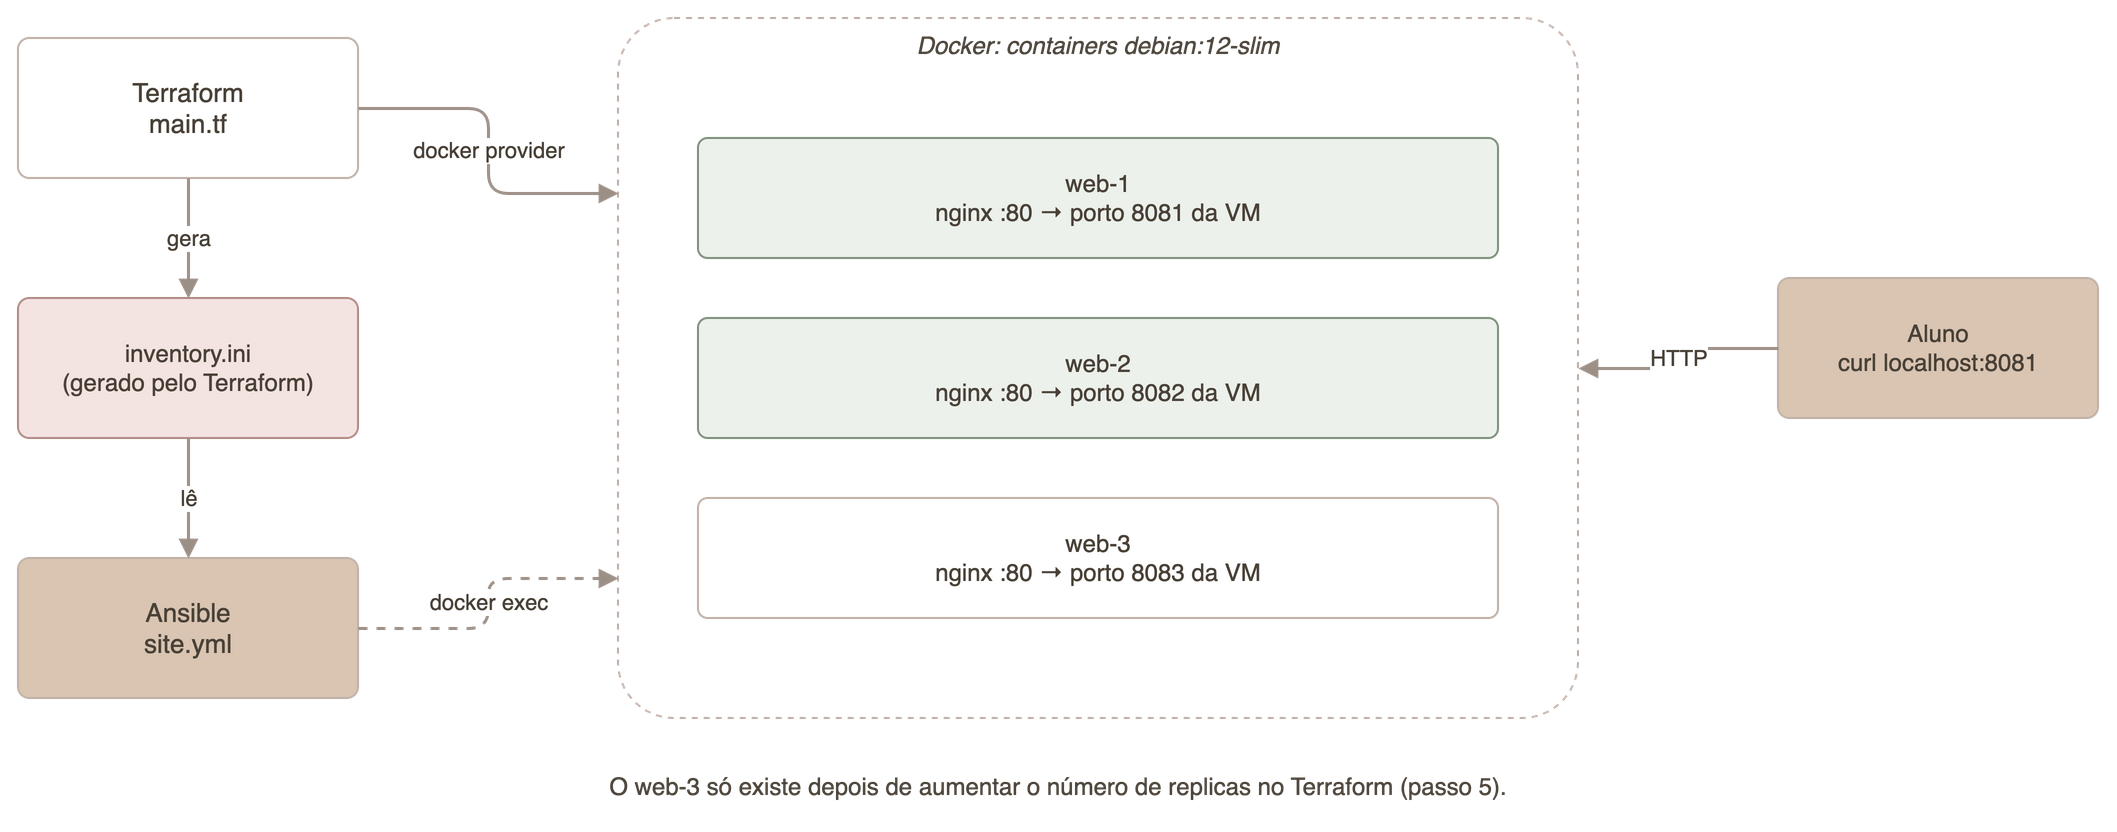
\includegraphics[width=\linewidth]{../Diagramas/g07-topologia.png}
\end{center}

\begin{leitura}
À esquerda estão as três peças de código. O Terraform, em cima, cria os containers através do provider do Docker e gera o ficheiro \cmd{inventory.ini}. O Ansible, em baixo, lê esse inventory e executa o playbook em cada container com \cmd{docker exec}, representado a tracejado. A caixa central contém os containers: o \cmd{web-1} e o \cmd{web-2} a verde existem desde o passo 4, e o \cmd{web-3} a branco só passa a existir quando se aumentar o número de replicas. À direita, o aluno testa cada servidor com \cmd{curl} através do porto correspondente da máquina virtual.
\end{leitura}

\begin{teoria}
Um container novo não tem Python, e o Ansible precisa dele no host para executar a maioria dos módulos. Esta é a contrapartida do modelo agentless: não há agente, mas há requisitos mínimos. O primeiro play usa o módulo \cmd{raw}, que executa um comando sem depender de Python, para instalar o interpretador. Só depois se usam os módulos habituais.

A ligação ao container usa o \emph{connection plugin} \cmd{community.docker.docker}, em vez do SSH. O resto do Ansible é igual: inventory, playbook, tasks e handlers. Isto mostra que o Ansible é independente do transporte.

Neste passo, deve analisar-se quais os hosts que o Ansible altera quando o Terraform acrescenta um container.
\end{teoria}

\subsection*{5.1 O inventory gerado pelo Terraform}

Acrescentar ao fim do \cmd{main.tf} o recurso que gera o inventory e uma saída com os endereços:

\begin{ficheiro}{main.tf (acrescentar ao fim)}
resource "local_file" "inventory" {
  filename = "${path.module}/inventory.ini"
  content  = templatefile("${path.module}/inventory.tftpl", {
    nomes = docker_container.web[*].name
  })
}

output "urls" {
  value = [for c in docker_container.web : "http://localhost:${c.ports[0].external}"]
}
\end{ficheiro}

\begin{ficheiro}{inventory.tftpl}
[web]
%{ for nome in nomes ~}
${nome} ansible_connection=community.docker.docker
%{ endfor ~}
\end{ficheiro}

\begin{terminal}
terraform init
terraform apply -auto-approve
cat inventory.ini
\end{terminal}

\begin{saida}
Apply complete! Resources: 1 added, 0 changed, 0 destroyed.
urls = ["http://localhost:8081", "http://localhost:8082"]

[web]
web-1 ansible_connection=community.docker.docker
web-2 ansible_connection=community.docker.docker
\end{saida}

\subsection*{5.2 O playbook para os containers}

\begin{ficheiro}{ansible.cfg}
[defaults]
inventory = terraform/inventory.ini
host_key_checking = False
interpreter_python = auto_silent
\end{ficheiro}

\begin{ficheiro}{site.yml}
- name: Preparar os hosts (Python)
  hosts: web
  gather_facts: false
  tasks:
    - name: Instalar o Python se nao existir
      ansible.builtin.raw: >
        test -x /usr/bin/python3 ||
        (apt-get update -qq && apt-get install -y -qq python3 python3-apt)
      changed_when: false

- name: Configurar os servidores web
  hosts: web
  tasks:
    - name: Instalar o nginx
      ansible.builtin.apt:
        name: nginx
        state: present
        update_cache: true
        cache_valid_time: 3600
    - name: Gerar a pagina inicial a partir do template
      ansible.builtin.template:
        src: index.html.j2
        dest: /var/www/html/index.nginx-debian.html
        mode: "0644"
      notify: Recarregar o nginx
    - name: Arrancar o nginx
      ansible.builtin.command: nginx
      args:
        creates: /run/nginx.pid
  handlers:
    - name: Recarregar o nginx
      ansible.builtin.command: nginx -s reload
\end{ficheiro}

\begin{nota}
Os ficheiros \cmd{ansible.cfg}, \cmd{site.yml} e \cmd{index.html.j2} ficam em \cmd{\textasciitilde/icn-aula07}, e o comando \cmd{ansible-playbook} deve ser executado a partir desse diretório. O \cmd{main.tf} e o inventory ficam em \cmd{\textasciitilde/icn-aula07/terraform}.
\end{nota}

\subsection*{5.3 Execução}

\begin{terminal}
cd ~/icn-aula07
ansible-playbook site.yml
curl -s localhost:8081
curl -s localhost:8082
\end{terminal}

\begin{saida}
PLAY RECAP
web-1 : ok=4  changed=3  unreachable=0  failed=0
web-2 : ok=4  changed=3  unreachable=0  failed=0
<h1>Aula 07 - IaC</h1>
<p>Servidor web-2 com Debian 12</p>
\end{saida}

\begin{erro}
Se o Ansible indicar que a ligação ao container falhou, confirmar que o nome no inventory coincide com o resultado de \cmd{docker ps}. Se aparecer uma mensagem sobre a coleção \cmd{community.docker}, instalar com \cmd{ansible-galaxy collection install community.docker}.
\end{erro}

\subsection*{5.4 Escalar e reconfigurar}

Aumentar o número de replicas no Terraform, regenerar o inventory e voltar a executar o playbook:

\begin{terminal}
cd ~/icn-aula07/terraform
terraform apply -auto-approve -var replicas=3
cd ~/icn-aula07
ansible-playbook site.yml
curl -s localhost:8083
\end{terminal}

\begin{saida}
web-1 : ok=3  changed=0  unreachable=0  failed=0
web-2 : ok=3  changed=0  unreachable=0  failed=0
web-3 : ok=4  changed=3  unreachable=0  failed=0
<p>Servidor web-3 com Debian 12</p>
\end{saida}

\begin{observe}
O \cmd{web-1} e o \cmd{web-2} reportam \emph{changed=0}: já estavam conforme, e o Ansible não lhes tocou. Só o \cmd{web-3}, novo, foi configurado. A mudança de infraestrutura foi feita num valor (\cmd{replicas}), e a configuração seguiu-a sem alterar o playbook. Qual seria o trabalho equivalente se os servidores fossem configurados à mão?
\end{observe}

\begin{feito}
O \cmd{curl} responde nos três portos (8081, 8082 e 8083) com a página gerada pelo template, e a segunda execução do playbook não alterou os servidores já existentes.
\end{feito}

\passo{6}{Gestão de segredos com o Ansible Vault}

\textbf{Objetivo.} Cifrar uma credencial com o Ansible Vault, verificar que não fica legível no ficheiro e usá-la num playbook sem a expor.

\textbf{Enquadramento.} O código de infraestrutura vai para o Git, mas as passwords não podem ir com ele em texto simples. A aula apresentou o Ansible Vault como uma das soluções, e este passo mostra o seu funcionamento.

\begin{teoria}
O Ansible Vault cifra ficheiros de variáveis com uma palavra-passe. O ficheiro cifrado pode ser guardado no repositório, porque o seu conteúdo só é legível por quem conhece a palavra-passe. Na execução, o Ansible pede a palavra-passe, decifra em memória e usa as variáveis como quaisquer outras.

Numa task que manipula o segredo, a opção \cmd{no\_log} impede que o valor apareça na saída do Ansible e nos registos.

Neste passo, deve analisar-se o aspeto do ficheiro cifrado e o que o Ansible mostra, e não mostra, durante a execução.
\end{teoria}

\subsection*{6.1 Criação do ficheiro cifrado}

\begin{terminal}
cd ~/icn-aula07
ansible-vault create segredos.yml
\end{terminal}

O Ansible pede uma palavra-passe para o cofre, que deve ser fornecida duas vezes (neste laboratório pode usar-se uma palavra-passe simples, por exemplo \cmd{icn2026}). Abre-se depois um editor, onde se escreve:

\begin{ficheiro}{segredos.yml (dentro do editor)}
db_password: "palavra-passe-da-base-de-dados"
\end{ficheiro}

Guardar e sair do editor. Observar o conteúdo do ficheiro tal como fica no disco:

\begin{terminal}
cat segredos.yml
\end{terminal}

\begin{saida}
$ANSIBLE_VAULT;1.1;AES256
6338613161633531...
\end{saida}

\subsection*{6.2 Utilização no playbook}

\begin{ficheiro}{segredo.yml}
- name: Usar um segredo cifrado
  hosts: web
  gather_facts: false
  vars_files:
    - segredos.yml
  tasks:
    - name: Gravar o segredo no container
      ansible.builtin.copy:
        content: "{{ db_password }}"
        dest: /etc/app-secret
        mode: "0600"
      no_log: true
\end{ficheiro}

\begin{terminal}
ansible-playbook segredo.yml --ask-vault-pass
docker exec web-1 cat /etc/app-secret
\end{terminal}

\begin{saida}
Vault password:
TASK [Gravar o segredo no container] ... changed: [web-1]
palavra-passe-da-base-de-dados
\end{saida}

\begin{erro}
Se a execução falhar com \cmd{Attempting to decrypt but no vault secrets found}, faltou a opção \cmd{-{}-ask-vault-pass}. Se falhar com \cmd{Decryption failed}, a palavra-passe introduzida é diferente da usada na criação do ficheiro.
\end{erro}

\begin{observe}
O ficheiro \cmd{segredos.yml} pode ser guardado no repositório, porque o conteúdo é ilegível sem a palavra-passe. A saída do playbook não mostra o valor do segredo, graças ao \cmd{no\_log}. Num cenário real, a palavra-passe do cofre seria injetada pelo sistema de CI/CD e nunca escrita no repositório.
\end{observe}

\begin{feito}
O ficheiro \cmd{segredos.yml} começa por \cmd{\$ANSIBLE\_VAULT} e o container contém o segredo em \cmd{/etc/app-secret}.
\end{feito}

\passo{7}{Limpeza}

\textbf{Objetivo.} Destruir os recursos criados e apagar a máquina virtual, libertando memória e disco.

\textbf{Enquadramento.} Tal como a criação, a destruição é declarativa: o Terraform conhece tudo o que criou, através do state file, e remove exatamente isso.

\subsection*{7.1 Destruição dos recursos}

\begin{terminal}
cd ~/icn-aula07/terraform
terraform destroy -auto-approve
docker ps -a
\end{terminal}

\begin{saida}
Destroy complete! Resources: 5 destroyed.
CONTAINER ID   IMAGE   COMMAND   CREATED   STATUS   PORTS   NAMES
\end{saida}

\subsection*{7.2 Eliminação da máquina virtual}

Sair da máquina virtual e, no computador do aluno, apagá-la:

\begin{terminal}
exit
multipass delete icn-iac
multipass purge
multipass list
\end{terminal}

\begin{saida}
No instances found.
\end{saida}

\begin{feito}
O comando \cmd{multipass list} não apresenta a instância \cmd{icn-iac}.
\end{feito}

\section*{Problemas frequentes}

\begin{center}
\small
\begin{tabular}{>{\raggedright\arraybackslash}p{6.4cm} >{\raggedright\arraybackslash}p{8.4cm}}
\toprule
\textbf{Sintoma} & \textbf{Resolução} \\
\midrule
\cmd{permission denied} no Docker & Sair e entrar de novo na máquina virtual para ativar o grupo \cmd{docker}. \\
YAML rejeitado pelo Ansible & Substituir tabulações por espaços e rever a indentação. \\
\cmd{terraform init} falha & Verificar a ligação à Internet e repetir. \\
Porto 8081 ocupado & Identificar o processo com \cmd{sudo ss -ltnp} e terminá-lo. \\
Ansible sem Python no container & Executar primeiro o play de preparação do \cmd{site.yml}. \\
Esqueceu a palavra-passe do cofre & Criar novo \cmd{segredos.yml}; o ficheiro cifrado não é recuperável. \\
\bottomrule
\end{tabular}
\end{center}

\section*{Comandos utilizados}

\begin{center}
\small
\begin{tabular}{>{\raggedright\arraybackslash}p{7cm} >{\raggedright\arraybackslash}p{7.8cm}}
\toprule
\textbf{Comando} & \textbf{Finalidade} \\
\midrule
\cmd{multipass launch 22.04 -{}-name icn-iac} & Criar a máquina virtual \\
\cmd{ansible localhost -m lineinfile} & Executar um módulo isolado (ad hoc) \\
\cmd{ansible-playbook playbook.yml} & Executar um playbook \\
\cmd{ansible-playbook -{}-check -{}-diff} & Mostrar as alterações sem as aplicar \\
\cmd{ansible-vault create ficheiro.yml} & Criar um ficheiro cifrado \\
\cmd{terraform init} & Obter os providers \\
\cmd{terraform plan} & Mostrar as alterações previstas \\
\cmd{terraform apply} & Executar as alterações \\
\cmd{terraform state list} & Listar os recursos no state file \\
\cmd{terraform destroy} & Destruir os recursos \\
\cmd{docker ps} & Listar os containers em execução \\
\cmd{multipass delete icn-iac} & Apagar a máquina virtual \\
\bottomrule
\end{tabular}
\end{center}

\section*{Questões de consolidação}

As questões seguintes destinam-se a discussão e não têm de ser entregues.

\begin{enumerate}
  \item Porque é que o ficheiro imperativo ficou com duas linhas e o declarativo com uma? Que propriedade explica a diferença?
  \item O que distingue o resultado \emph{changed} do resultado \emph{ok}, e porque é que é útil conhecê-lo?
  \item Em que se assemelham o \cmd{terraform plan} e o \cmd{ansible-playbook -{}-check -{}-diff}? Em que diferem?
  \item Qual é o papel do state file? O que aconteceria ao Terraform se o ficheiro fosse apagado?
  \item Porque é que, ao passar de dois para três containers, o Ansible só alterou o \cmd{web-3}?
  \item Porque é que o ficheiro \cmd{segredos.yml} pode ser guardado no Git, e que cuidado exige a palavra-passe do cofre?
\end{enumerate}

\section*{Síntese}

O laboratório permitiu observar, na prática, as ideias centrais da Aula 07:

\begin{itemize}
  \item Um script \textbf{imperativo} repete os passos, e um módulo \textbf{declarativo} só atua quando há diferença: é a \textbf{idempotência}.
  \item O Ansible \textbf{configura} o que corre dentro de uma máquina e distingue o que mudou (\emph{changed}) do que já estava conforme (\emph{ok}).
  \item O \textbf{drift} é detetado e corrigido por nova execução, tanto no Ansible como no Terraform.
  \item O Terraform \textbf{provisiona} recursos, mostra o plano antes de o aplicar e regista o resultado no \textbf{state file}.
  \item As duas camadas ligam-se por um \textbf{inventory} gerado pelo Terraform: alterar um valor no código basta para escalar e reconfigurar.
  \item Um \textbf{segredo} cifrado com o Ansible Vault pode viver no repositório sem ficar exposto.
\end{itemize}

\end{document}
